\section{Introduction to the queue}
\begin{itemize}
    \item The queue is similar to the stack, however, the queue follows the first in first out order.
    \item The queue data structure has two ends, front end and the back end.
    \item Front end is the end where the elements are deleted.
    \item Back end is where the elements are inserted.
    \item FIFO: First In First Out. 
    \item In the stack, we only had une end in which we performed all the operations, we poped from the top, and inserted in the top. 
    \item In the queue we have two ends in which we can perform operations, back end and the front end, back end is for inserting and front end is for deleting. 
\end{itemize}

\subsection{Formal definition}
\begin{itemize}
    \item Queue: Queue is a linear data structure with two open ends, called the ``rear'' and the ``front'', elements are added at the ``rear'' end and deleted from the ``front'' end. 
    \item The term linear data structure implies that the data structure has no hierarchical order. A tree is a hierarchical data structure, queue is not a hierarchical data structure. 
    \item Elements in a queue typically follows ``First In First Out'' order, that is elements inserted first will be always deleted first. 
    \item Also called FIFO data structure. 
\end{itemize}

\subsection{Some other variations of the queue data structure}
\begin{itemize}
    \item Double ended queue: elements can added or deleted form both ends, this means from the rear and the front. It's a mixture of FIFO and LIFO. 
    \item Priority queue: elements are deleted on the basis of predefined priority. In the FIFO queue the priority in deleting is always found in the front. Consider a situation in which an interview is being granted to potential students applying for a job, students are standing in a line following the FIFO order, when the interviewer comes in, he decides he no longer wants the FIFO order and instead wants the highest grade to pass first, this is a priority for the higher grade students. The queue transforms in to a priority queue. 
        \begin{itemize}
            \item This can be implemented using a heap data structure.
        \end{itemize}
\end{itemize}


%----------------------------------------------------------------------------------------
\section{The FIFO queue implementation idea using array}
\begin{itemize}
    \item We start declaring an array, in the initialization, the rear and the front end will be the same. 
        \begin{figure}[H]
            \centering
            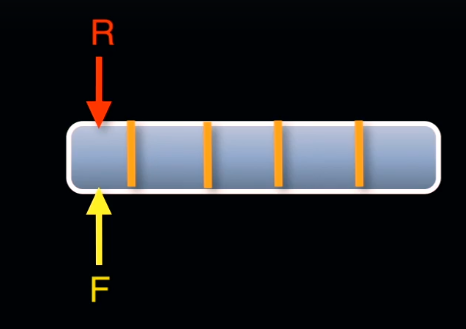
\includegraphics[width=7cm]{\figs/queue_1.png} 
        \end{figure}
    
    \item Now the equivalent of inserting in a queue is called enqueue, and the equivalent of deletion is dequeue. We now enqueue \mintinline{c}{'A'} to the queue.
        \begin{minted}[autogobble]{c}
            Queue.enqueue('A');
        \end{minted}
        \begin{figure}[H]
            \centering
            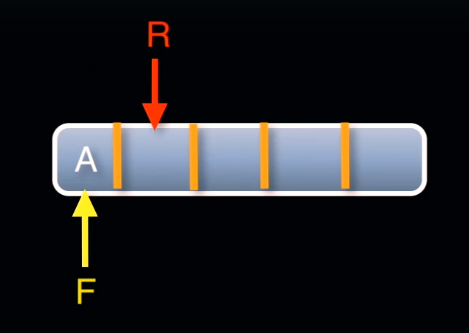
\includegraphics[width=7cm]{\figs/queue_2.png} 
        \end{figure}
    
    \item We enqueue \mintinline{c}{'B'}.
        \begin{minted}[autogobble]{c}
            Queue.enqueue('B');
        \end{minted}
        \begin{figure}[H]
            \centering
            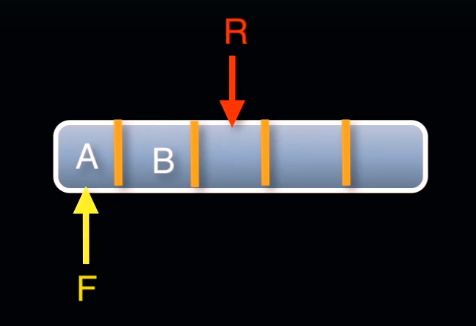
\includegraphics[width=7cm]{\figs/queue_3.png} 
        \end{figure}
    
    \item We enqueue \mintinline{c}{'C'}.
        \begin{minted}[autogobble]{c}
            Queue.enqueue('C');
        \end{minted}
        \begin{figure}[H]
            \centering
            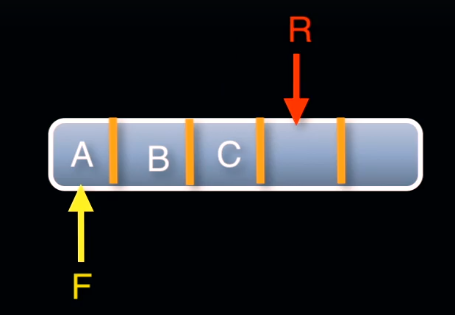
\includegraphics[width=7cm]{\figs/queue_4.png} 
        \end{figure}
    
    \item We now dequeue.
        \begin{minted}[autogobble]{c}
            Queue.dequeue();
        \end{minted}
        \begin{figure}[H]
            \centering
            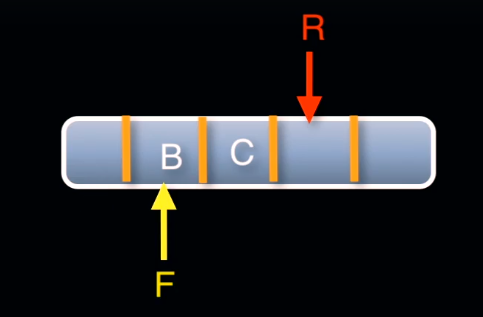
\includegraphics[width=7cm]{\figs/queue_5} 
        \end{figure}
        
    \item We dequeue.
        \begin{minted}[autogobble]{c}
            Queue.dequeue();
        \end{minted}
        \begin{figure}[H]
            \centering
            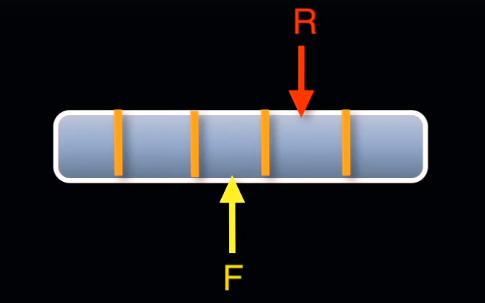
\includegraphics[width=7cm]{\figs/queue_6} 
        \end{figure}
    
    \item We are now at an underflow state.
        \begin{minted}[autogobble]{c}
            Queue.dequeue();
        \end{minted}
        \begin{figure}[H]
            \centering
            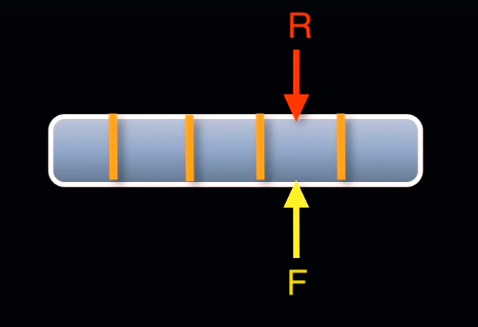
\includegraphics[width=7cm]{\figs/queue_7} 
        \end{figure}
    
    \item We can enqueue again.
        \begin{minted}[autogobble]{c}
            Queue.enqueue('X');
        \end{minted}
        \begin{figure}[H]
            \centering
            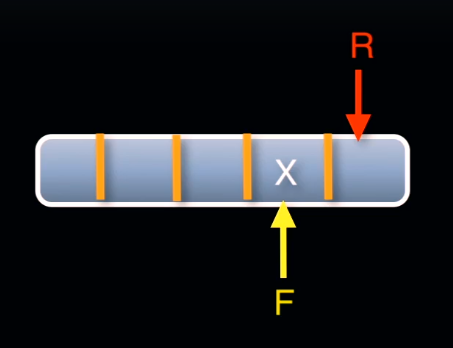
\includegraphics[width=7cm]{\figs/queue_8} 
        \end{figure}
\end{itemize}


%----------------------------------------------------------------------------------------
\section{Algorithm for FIFO Queue}

Initial declarations: 
\begin{center}
    \begin{itemize}
        \item REAR: is an integer value to hold the index of the rear end of Q, that is the index of the next insertion element. 
        \item FRONT: is an integer variable to hold the index of the front end of Q, that is the index of the next element to be deleted. 
        \item ITEM[SIZE]: is a 1-D array that we will be using for keeping the queue elements SIZE is the size of the queue, that is the number of elements in the array, we consider the index of the array starts from 0.
        \item Initially: 
            \begin{lstlisting}
                REAR = 0; 
                FRONT = 0;
            \end{lstlisting}
        
        \item Underflow condition: if the rear and front are equal then this the condition for underflow checking, this means the queue is empty. 
        \item Overflow condition: when the rear index goes beyond the last element. When the rear is equal to the size.
        \item Enqueue: place the new element at the rear index and then move the rear to the next element. If the rear goes beyond the last element that means we have inserted the new element in the last index, we can't insert anymore, this will cause an overflow.
        \item Dequeue: remove the front element and move the front forward by one. 
    \end{itemize}
\end{center}

\subsection{Enqueue}
\begin{algorithm}[H]
    \SetAlgoLined
    % \DontPrintSemiColon
    OPERATION ENQUEUE (v)
    % \Input{v}
    \BlankLine
    \large
    \If{rear == SIZE}{
        print "Queue overflow"\;
        exit queue\; 
    }
    
    item[rear] = v\; 
    rear = rear + 1\; 
    \caption{OPERATION ENQUEUE (v)}
\end{algorithm}

\subsection{Dequeue}
\begin{center}
    \begin{algorithm}[H]
        \SetAlgoLined
        % \DontPrintSemiColon
        % \Input{}
        % \Output{}
        % \BlankLine
        \large
        \If{rear == front}{
            print "Queue underflow"\;
            exit dequeue\;
        }
        v = item[front]\; 
        front = front + 1\; 
        return v\; 
        \caption{OPERATION DEQUEUE (v)}
    \end{algorithm}
\end{center}    


%----------------------------------------------------------------------------------------
\section{Implementation of  FIFO Queue}
\inputcode{c}{\code/implementation_queue.c}

\section{The loophole in our implementation of FIFO queue}
\begin{itemize}
    \item The queue can't be reused essentially, enqueing 3 elements and then dequeueing them inserts new elements in the third. 
    \item Changing the item memeber size to 5 for practical reasons. 
        \begin{minted}[autogobble]{c}
            #define SIZE 5
        \end{minted}
    
    \item We can observe that eventually the queue will be in a state of overflow and underflow at the same time with the user not being able to do anything to help it. 
        \begin{minted}[autogobble]{c}
            /* Output: 
            ----Queue operations----
            1. Enqueue
            2. Dequeue
            3. Quit
            --------------------------
            Input your option: 1
            Input the value to enqueue: 100
            Input your option: 1
            Input the value to enqueue: 200
            Input your option: 1
            Input the value to enqueue: 300
            Input your option: 1
            Input the value to enqueue: 400
            Input your option: 2
            Deleted value: 100
            Input your option: 2
            Deleted value: 200
            Input your option: 2
            Deleted value: 300
            Input your option: 2
            Deleted value: 400
            Input your option: 2
            Queue underflow
            Input your option: 1
            Input the value to enqueue: 500
            Input your option: 1
            Input the value to enqueue: 600
            Queue overflow
            Input your option: 3
            */
        \end{minted}
\end{itemize}


%----------------------------------------------------------------------------------------
\section{Understanding the loophole, why it happens?}
\begin{itemize}
    \item The solution lies in the rear and the front to be relocated to the beginning of the array. 
    \item This is called a circular queue.
\end{itemize}


%----------------------------------------------------------------------------------------
\section{Introduction to circular queue}
\begin{itemize}
    \item We have a queue, instead of moving the front  and rear in the way a normal queue operates, we will use the following formulas:
        \[
          r = (r+1)\%\text{ SIZE }
        \]
        \[
          p = (p+1)\%\text{ SIZE }
        \]
    
    \item You can also use if-else statements to do the same thing:
        \begin{center}
            \begin{algorithm}[H]
                \SetAlgoLined
                % \DontPrintSemiColon
                % \Input{}
                % \Output{}
                % \BlankLine
                \large
                \eIf{rear == size - 1}{
                    r = 0\;
                }{
                    r++\;
                }
                \caption{Perform a cricular queue}
            \end{algorithm}
        \end{center}
\end{itemize}


%----------------------------------------------------------------------------------------
\section{Circular queue operations}
\begin{center}
    \begin{itemize}
        \item Let's suppose that we start at an underflow condition.
        \item REAR = SIZE - 1 
        \item FRONT = SIZE - 1
        \item SIZE = 5
    \end{itemize}
    \begin{tabular}{ cc }
        {R$\rightarrow$}&{4} \\ {}&{3} \\ {}&{2} \\ {}&{1} \\ {}&{0} \\
    \end{tabular}
    \begin{tabular}{|p{0.75cm}|}
        \hline {} \\ \hline {} \\ \hline {} \\ \hline {} \\ \hline {} \\ \hline
    \end{tabular}
    \begin{tabular}{ c }
        {$\leftarrow$F} \\ {} \\ {} \\ {} \\ {} \\
    \end{tabular}

    \begin{minted}[autogobble]{c}
        CircularQueue.enqueue(5);
        // Increase the rear: r = (4+1)%5 -> 0
    \end{minted}

    \begin{tabular}{ cc }
        {}&{4} \\ {}&{3} \\ {}&{2} \\ {}&{1} \\ {R$\rightarrow$}&{0} \\
    \end{tabular}
    \begin{tabular}{|p{0.75cm}|}
        \hline {} \\ \hline {} \\ \hline {} \\ \hline {} \\ \hline {5} \\ \hline
    \end{tabular}
    \begin{tabular}{ c }
        {$\leftarrow$F} \\ {} \\ {} \\ {} \\ {} \\
    \end{tabular}

    \begin{minted}[autogobble]{c}
        CirucularQueue.enqueue(10);
        // rear: (5+1)%5 = 1
    \end{minted}

    \begin{tabular}{ cc }
        {}&{4} \\ {}&{3} \\ {}&{2} \\ {R$\rightarrow$}&{1} \\ {}&{0} \\
    \end{tabular}
    \begin{tabular}{|p{0.75cm}|}
        \hline {} \\ \hline {} \\ \hline {} \\ \hline {10} \\ \hline {5} \\ \hline
    \end{tabular}
    \begin{tabular}{ c }
        {$\leftarrow$F} \\ {} \\ {} \\ {} \\ {} \\
    \end{tabular}

    \begin{minted}[autogobble]{c}
        CircularQueue.enqueue(15);
        // rear\alpha (6+1)%5 = 2
    \end{minted}

    \begin{tabular}{ cc }
        {}&{4} \\ {}&{3} \\ {R$\rightarrow$}&{2} \\ {}&{1} \\ {}&{0} \\
    \end{tabular}
    \begin{tabular}{|p{0.75cm}|}
        \hline {} \\ \hline {} \\ \hline {15} \\ \hline {10} \\ \hline {5} \\ \hline
    \end{tabular}
    \begin{tabular}{ c }
        {$\leftarrow$F} \\ {} \\ {} \\ {} \\ {} \\
    \end{tabular}

    \begin{minted}[autogobble]{c}
        CircularQueue.enqueue(20);
        // rear: (7+1)%5 = 3
    \end{minted}

    \begin{tabular}{ cc }
        {}&{4} \\ {R$\rightarrow$}&{3} \\ {}&{2} \\ {}&{1} \\ {}&{0} \\
    \end{tabular}
    \begin{tabular}{|p{0.75cm}|}
        \hline {} \\ \hline {20} \\ \hline {15} \\ \hline {10} \\ \hline {5} \\ \hline
    \end{tabular}
    \begin{tabular}{ c }
        {$\leftarrow$F} \\ {} \\ {} \\ {} \\ {} \\
    \end{tabular}

    \begin{itemize}
        \item An error will occur because in the next insertion will satisfy the underflow condition (rear == front).
    \end{itemize}
    \begin{minted}[autogobble]{c}
        CircularQueue.enqueue(25);
        // rear: (8+1)%5 = 4
    \end{minted}
    \begin{itemize}
        \item This operation will enter the if statement of the queue underflow.
            \begin{minted}[autogobble]{c}
                if (rear == front){
                    printf("Underflow");
                }
            \end{minted}
        
        \item The insertion will never happen. 
        \item We need to dequeue the last value at index 4.
        \begin{minted}[autogobble]{c}
            CircularQueue.dequeue();
            // This will set the front back to 0
            // f = (f+1)%SIZE: (4+1)%5 = 0
        \end{minted}
    \end{itemize}
    \begin{tabular}{ cc }
        {}&{4} \\ {R$\rightarrow$}&{3} \\ {}&{2} \\ {}&{1} \\ {}&{0} \\
    \end{tabular}
    \begin{tabular}{|p{0.75cm}|}
        \hline {} \\ \hline {20} \\ \hline {15} \\ \hline {10} \\ \hline {5} \\ \hline
    \end{tabular}
    \begin{tabular}{ c }
        {} \\ {} \\ {} \\ {} \\ {$\leftarrow$F} \\
    \end{tabular}
    

    \begin{itemize}
        \item Now we can move the rear to the next element without satisfying the underflow condition (front == rear).
        \item The queue is now at an overflow state.
    \end{itemize}
    \begin{minted}[autogobble]{c}
        CircularQueue.enqueue(25);
        // rear: 
    \end{minted}
    \begin{itemize}
        \item You can't enqueue anymore because all are occupied. 
    \end{itemize}
    \begin{tabular}{ cc }
        {R$\rightarrow$}&{4} \\ {}&{3} \\ {}&{2} \\ {}&{1} \\ {}&{0} \\
    \end{tabular}
    \begin{tabular}{|p{0.75cm}|}
        \hline {25} \\ \hline {20} \\ \hline {15} \\ \hline {10} \\ \hline {5} \\ \hline
    \end{tabular}
    \begin{tabular}{ c }
        {} \\ {} \\ {} \\ {} \\ {$\leftarrow$F} \\
    \end{tabular}
\end{center}



%----------------------------------------------------------------------------------------
\section{Algorithms for enqueue and dequeue operations for a circular queue}

\subsection{Enqueue}
\begin{center}
    \begin{itemize}
        \item Initially: item is a 1-D array to hold the queue elements.
    \end{itemize}
    \begin{algorithm}[H]
        \SetAlgoLined
        % \DontPrintSemiColon
        % \Input{}
        % \Output{}
        % \BlankLine
        \large
        rear = SIZE - 1\; 
        front = SIZE - 1\;  
        \If{(rear + 1) \% SIZE == front}{
            print "Queue overflow"\; 
            exit ENQUEUE\; 
        }
        rear = (rear + 1) \% SIZE\;
        item[rear] = v\;  
        END ENQUEUE\; 
        \caption{OPERATION ENQUEUE(v)}
    \end{algorithm}
\end{center}

\subsection{Dequeue}
\begin{center}
    \begin{algorithm}[H]
        \SetAlgoLined
        % \DontPrintSemiColon
        % \Input{}
        % \Output{}
        % \BlankLine
        \large
        \If{rear == front}{
            print "Queue underflow"\; 
            exit DEQUEUE\; 
        }
        front = (front + 1) \% SIZE\; 
        v = item[front]\; 
        return v\; 
        END DEQUEUE\; 
        \caption{OPERATION DEQUEUE}
    \end{algorithm}
\end{center}


%----------------------------------------------------------------------------------------
\section{Implementation of Circular Queue}
\inputcode{c}{\code/implementation_of_circular_queue.c}


%----------------------------------------------------------------------------------------
\section{Introduction to Double Ended Queue}
\begin{itemize}
    \item In a double ended queue, you can insert or delete front either side of the queue, it's a mixture of the stack and FIFO queue data structure. 
    \item The operations are:
        \begin{itemize}
            \item Inserting at REAR.
            \item Deletion from REAR.
            \item Inserting at FRONT.
            \item Deleting from FRONT. 
        \end{itemize}
\end{itemize}

\subsection{Example}
    
\begin{itemize}
    \item Insertion at REAR.
        \begin{itemize}
            \item Inserting at rear and deleting from rear are exactly the same as the push and pop operations we had in the stack.
            \item Assume:
                \begin{itemize}
                    \item REAR = -1
                    \item FRONT = 0
                \end{itemize}
        \end{itemize}
        \begin{center}
            \begin{tabular}{ |p{6cm}|p{6cm}| }

                \hline
                \vspace{0.1cm}
                \begin{tabular}{ cc }
                    {}&{4} \\ {}&{3} \\ {}&{2} \\ {}&{1} \\ {F$\rightarrow$}&{0} \\ {}&{}\\
                \end{tabular}
                \begin{tabular}{|p{0.75cm}|}
                    \hline {} \\ \hline {} \\ \hline {} \\ \hline {} \\ \hline {} \\ \hline \multicolumn{1}{c}{} \\
                \end{tabular}
                \begin{tabular}{ c }
                    {} \\ {} \\ {} \\ {} \\ {} \\ {$\leftarrow$R=-1} \\ 
                \end{tabular}
                {
                    \begin{itemize}
                        \item The DEQueue is empty and the rear is in -1 and front is in 0.
                    \end{itemize}
                }
                & 
                \vspace{0.1cm}
                \begin{tabular}{ cc }
                    {}&{4} \\ {}&{3} \\ {}&{2} \\ {}&{1} \\ {F$\rightarrow$}&{0} \\ {}&{}\\
                \end{tabular}
                \begin{tabular}{|p{0.75cm}|}
                    \hline {} \\ \hline {} \\ \hline {} \\ \hline {} \\ \hline {12} \\ \hline \multicolumn{1}{c}{} \\
                \end{tabular}
                \begin{tabular}{ c }
                    {} \\ {} \\ {} \\ {} \\ {$\leftarrow$R=0} \\ {} \\ 
                \end{tabular}
                {
                    \begin{minted}[autogobble]{c}
                        DEQueue.insertAtRear(12);
                    \end{minted}
                }

                \\ \hline
                \vspace{0.1cm}
                \begin{tabular}{ cc }
                    {}&{4} \\ {}&{3} \\ {}&{2} \\ {}&{1} \\ {F$\rightarrow$}&{0} \\ {}&{}\\
                \end{tabular}
                \begin{tabular}{|p{0.75cm}|}
                    \hline {} \\ \hline {} \\ \hline {} \\ \hline {} \\ \hline {12} \\ \hline \multicolumn{1}{c}{} \\
                \end{tabular}
                \begin{tabular}{ c }
                    {} \\ {} \\ {} \\ {} \\ {$\leftarrow$R=0} \\ {} \\ 
                \end{tabular}

                & 
                \vspace{0.1cm}
                \begin{tabular}{ cc }
                    {}&{4} \\ {}&{3} \\ {}&{2} \\ {}&{1} \\ {F$\rightarrow$}&{0} \\ {}&{}\\
                \end{tabular}
                \begin{tabular}{|p{0.75cm}|}
                    \hline {} \\ \hline {} \\ \hline {} \\ \hline {14} \\ \hline {12} \\ \hline \multicolumn{1}{c}{} \\
                \end{tabular}
                \begin{tabular}{ c }
                    {} \\ {} \\ {} \\ {$\leftarrow$R=1} \\ {} \\ {} \\ 
                \end{tabular}
                {
                    \begin{minted}[autogobble]{c}
                        DEQueue.insertAtRear(14);
                    \end{minted}
                }       
                         
                \\ \hline

                \vspace{0.1cm}
                \begin{tabular}{ cc }
                    {}&{4} \\ {}&{3} \\ {}&{2} \\ {}&{1} \\ {F$\rightarrow$}&{0} \\ {}&{}\\
                \end{tabular}
                \begin{tabular}{|p{0.75cm}|}
                    \hline {} \\ \hline {} \\ \hline {15} \\ \hline {14} \\ \hline {12} \\ \hline \multicolumn{1}{c}{} \\
                \end{tabular}
                \begin{tabular}{ c }
                    {} \\ {} \\ {$\leftarrow$R=2} \\ {} \\ {} \\ {} \\ 
                \end{tabular}
                {
                    \begin{minted}[autogobble]{c}
                        DEQueue.insertAtRear(15);
                    \end{minted}
                }
                & 
                \vspace{0.1cm}
                \begin{tabular}{ cc }
                    {}&{4} \\ {}&{3} \\ {}&{2} \\ {}&{1} \\ {F$\rightarrow$}&{0} \\ {}&{}\\
                \end{tabular}
                \begin{tabular}{|p{0.75cm}|}
                    \hline {} \\ \hline {} \\ \hline {} \\ \hline {14} \\ \hline {12} \\ \hline \multicolumn{1}{c}{} \\
                \end{tabular}
                \begin{tabular}{ c }
                    {} \\ {} \\ {} \\ {$\leftarrow$R=1} \\ {} \\ {} \\ 
                \end{tabular}
                {
                    \begin{minted}[autogobble]{c}
                        DEQueue.deleteAtRear();
                    \end{minted}
                }
                \\ \hline
                
            \end{tabular}
        \end{center}
        \begin{itemize}
            \item The overflow condition for the insert at REAR is going to be when R=4.
        \end{itemize}
    
    \item Insertion at FRONT: when we have inserted with rear elements, and we have a situation in which the front is at index 0 and the rear is in index 2, when the rear is higher in terms of index than the front the insertion at FRONT will not be possible, this is the overflow condition.
    \item Perform deletions in a double ended queue, using the deletion from the FRONT.
        \begin{center}
            \begin{tabular}{ |p{6cm}|p{6cm}| }

                \hline
                \vspace{0.1cm}
                \begin{tabular}{ cc }
                    {}&{4} \\ {}&{3} \\ {}&{2} \\ {F$\rightarrow$}&{1} \\ {}&{0} \\ {}&{}\\
                \end{tabular}
                \begin{tabular}{|p{0.75cm}|}
                    \hline {} \\ \hline {} \\ \hline {} \\ \hline {14} \\ \hline {} \\ \hline \multicolumn{1}{c}{} \\
                \end{tabular}
                \begin{tabular}{ c }
                    {} \\ {} \\ {} \\ {$\leftarrow$R=1} \\ {} \\ {} \\ 
                \end{tabular}
                {
                    \begin{minted}[autogobble]{c}
                        DEQueue.deleteFromFront();
                        // deletes 12 and increments front by one
                    \end{minted}
                }
                & 
                \vspace{0.1cm}
                \begin{tabular}{ cc }
                    {}&{4} \\ {}&{3} \\ {F$\rightarrow$}&{2} \\ {}&{1} \\ {}&{0} \\ {}&{}\\
                \end{tabular}
                \begin{tabular}{|p{0.75cm}|}
                    \hline {} \\ \hline {} \\ \hline {} \\ \hline {} \\ \hline {} \\ \hline \multicolumn{1}{c}{} \\
                \end{tabular}
                \begin{tabular}{ c }
                    {} \\ {} \\ {} \\ {$\leftarrow$R=1} \\ {} \\ {} \\ 
                \end{tabular}
                {
                    \begin{minted}[autogobble]{c}
                        DEQueue.deleteFromFront();
                        // deletes 14 and increments front by one
                    \end{minted}
                }
                \\ \hline
            \end{tabular}
            \begin{itemize}
                \item Note that the queue is empty, we can not perform any more deletion.
                \item The underflow state happens when the front is greater than the rear. 
            \end{itemize}
        \end{center}
    
    \item Now lets try an insertion from the front.
        \begin{center}
            \begin{tabular}{ |p{6cm}|p{6cm}| }

                \hline
                \vspace{0.1cm}
                \begin{tabular}{ cc }
                    {}&{4} \\ {}&{3} \\ {}&{2} \\ {F$\rightarrow$}&{1} \\ {}&{0} \\ {}&{}\\
                \end{tabular}
                \begin{tabular}{|p{0.75cm}|}
                    \hline {} \\ \hline {} \\ \hline {} \\ \hline {10} \\ \hline {} \\ \hline \multicolumn{1}{c}{} \\
                \end{tabular}
                \begin{tabular}{ c }
                    {} \\ {} \\ {} \\ {$\leftarrow$R=1} \\ {} \\ {} \\ 
                \end{tabular}
                {
                    \begin{minted}[autogobble]{c}
                        DEQueue.insertAtFront(10);
                        // decrese the front by one and adds 10
                    \end{minted}
                }
                & 
                \vspace{0.1cm}
                \begin{tabular}{ cc }
                    {}&{4} \\ {}&{3} \\ {}&{2} \\ {}&{1} \\ {F$\rightarrow$}&{0} \\ {}&{}\\
                \end{tabular}
                \begin{tabular}{|p{0.75cm}|}
                    \hline {} \\ \hline {} \\ \hline {} \\ \hline {10} \\ \hline {20} \\ \hline \multicolumn{1}{c}{} \\
                \end{tabular}
                \begin{tabular}{ c }
                    {} \\ {} \\ {} \\ {$\leftarrow$R=1} \\ {} \\ {} \\ 
                \end{tabular}
                {
                    \begin{minted}[autogobble]{c}
                        DEQueue.insertAtFront(20);
                        // decrese the front by one and adds 20
                    \end{minted}
                }
                \\ \hline
                {
                    \begin{itemize}
                        \item Let's say we want to insert in the rear, this will be the procedure.
                    \end{itemize}
                }
                \vspace{0.1cm}
                \begin{tabular}{ cc }
                    {}&{4} \\ {}&{3} \\ {}&{2} \\ {}&{1} \\ {F$\rightarrow$}&{0} \\ {}&{}\\
                \end{tabular}
                \begin{tabular}{|p{0.75cm}|}
                    \hline {} \\ \hline {} \\ \hline {30} \\ \hline {10} \\ \hline {20} \\ \hline \multicolumn{1}{c}{} \\
                \end{tabular}
                \begin{tabular}{ c }
                    {} \\ {} \\ {$\leftarrow$R=2} \\ {} \\ {} \\ {} \\ 
                \end{tabular}
                {
                    \begin{minted}[autogobble]{c}
                        DEQueue.insertAtRear(30);
                        // increases rear by one and adds 30
                    \end{minted}
                }
                &
                \\ \hline
            \end{tabular}
        \end{center}
\end{itemize}



%----------------------------------------------------------------------------------------
\section{Algorithm development for double ended queue operations}
Take the following considerations:
\begin{itemize}
    \item FRONT = 0 
    \item REAR = -1
    \item SIZE = 5
\end{itemize}

\subsection{Insertion at rear}
\begin{center}
    \begin{algorithm}[H]
        \SetAlgoLined
        % \DontPrintSemiColon
        % \Input{}
        % \Output{}
        % \BlankLine
        \large

        \If{rear == SIZE - 1}{
            print "Unable to add at rear"\;
            exit INSERTION\_OPERATION\; 
        }
        rear = rear + 1\; 
        item[rear] = v\; 
        END INSERTION AT REAR\; 
        \caption{OPERATION INSERTION AT REAR (v)}
    \end{algorithm}
\end{center}

\subsection{Delete from rear}
\begin{center}
    \begin{algorithm}[H]
        \SetAlgoLined
        % \DontPrintSemiColon
        % \Input{}
        % \Output{}
        % \BlankLine
        \large
        \If{front $>$ rear}{
            print "Queue underflow"\; 
            exit DELETE FROM REAR\; 
        }
        v = item[rear]\; 
        rear = rear - 1\; 
        return v\; 
        END OF DELETE FROM REAR\; 
        \caption{OPERATION DELETE FROM REAR}
    \end{algorithm}
\end{center}

\subsection{Insert at front}
\begin{center}
    \begin{algorithm}[H]
        \SetAlgoLined
        % \DontPrintSemiColon
        % \Input{}
        % \Output{}
        % \BlankLine
        \large
        
        \If{front == 0}{
            print "Unable to insert at front"\; 
            exit OPERATION INSERT AT FRONT\; 
        }
        front = front - 1\; 
        item[front] = v\; 
        \caption{OPERATION INSERT AT FRONT}
    \end{algorithm}
\end{center}

\subsection{Deletion from front}
\begin{center}
    \begin{algorithm}[H]
        \SetAlgoLined
        % \DontPrintSemiColon
        % \Input{}
        % \Output{}
        % \BlankLine
        \large
        \If{front $>$ rear}{
            print "Queue underflow"\; 
            exit DELETE FROM FRONT\; 
        }
        v = item[front]\; 
        front = front + 1\; 
        return v\; 
        END DELETION FROM FRONT\; 
        \caption{OPERATION DELETION FROM FRONT}
    \end{algorithm}
\end{center}

\section{Implementation of double ended queue}
\inputcode{c}{\code/double_ended_queue.c}
